\begin{savequote}[75mm]
%``Keep it simple, stupid." (KISS doctrine)
%\qauthor{Clarence Leonard ``Kelly" Johnson - Lead Engineer at the Lockheed Skunk Works}
\end{savequote}

\chapter{Literature}

{\lettrine[lines=3,slope=1pt,nindent=1pt,]{\textcolor{SchoolColor}{T}}{he model in this paper} is influenced by several disciplines, including Urban Economics, Geography, Regional Science, Social Psychology, and Computational Sociology. While these disciplines are interested in modeling neighborhoods, they seem disconnected, evidenced by several paths and languages for identical or similar insights. For example, whereas regional science describes ``social energy''\cite{isard72}, economics has ``shadow prices,'' -- both of which provide the same argumentative work. Despite the unfortunate consequences of a failure to communicate between disciplines, there are still examples of insights unique to a single field. Hence, a multipronged approach may allow us to better reproduce the salient features of the housing market.

Most economists (and several researchers from other fields) study segregation through statistical regressions. The statistical regressions approach involves inferring relationships of raw data, indexes, and factors though statistical modeling based in some sort of regression analysis. However, to better capture the underlying mechanisms in housing markets, researchers need to model the problem more dynamically. Statistical modeling is very good at answering questions of correlation and significance. However, without some underlying theory in the model, statistical modeling is easily prone to spurious relationships and simple nonsense.  One alternative approach is structural econometric modeling, in which regressions are built around a theoretical model. A large number of mostly economic papers follow the Price Theory framework for their structural models, which constructs markets and economies of maximizing actors often with rational expectations.\footnote{Specifically, they model housing market through the work of Alonso 1964\cite{alonso64}, Mills (1967, 1972b)\cite{mills67,mills72a,mills72b}, and Muth 1969\cite{muth69}, which is built around optimizing the commuting cost differences within an urban area with the price of living there. The focus of of modeling this way, as Glen Weyl describes it, is:``an analysis that reduces rich (e.g. high-dimensional heterogeneity, many individuals) and often incompletely specified models into `prices’ sufficient to characterize approximate solutions to simple (e.g. one-dimensional policy) allocative problems." \cite{weyl15}. These price-theoretic papers model the dynamical nature of the economic system generally at the cost of complexity.} Price-theoretical models tend towards a Beckerian analysis in which the agents have a taste for discrimination and pay for it via opportunity cost. More recently, a small number of papers now follow the agent-based model (ABM) approach which may better capture the underlying dynamic process in housing markets. The ABM approach is built on simulations rather than regressions, but as a result it also requires a predictive economic model, thus also avoiding the pitfalls of simple regression analysis.  

Starting with Conway's ``Game of Life" in 1970 and Schelling's ``Dynamical models of segregation" in 1971, ABM models focus on using a foundation of simple rules to simulate complex behavior\cite{conway70,schelling71}. This is in contrast to the more traditional economic models, where the key modeling unit is a representative agent. ABM models allows the researcher to better focus on the heterogeneity within the system that may not be easily deduced by simply aggregating the properties of the agents. Additionally, in ABM models, the system in question is reduced to simple rules of interaction between agents and objects rather than mathematical equations that may be intractable or largely composed of florid distractions. In Conway's ``Game of Life'', there is simply a grid, two states for each box, and four simple rules. However, from even these simple simulations, complex behaviors can emerge. Several papers on evolutionary development, ecosystems, and swarming followed based on merely small changes to Conway's basic model. Schelling's segregation model, a similarly simple but powerful model, also provides the unfortunate insight that preventing segregation is a more difficult problem than originally thought. Even with simple rules for moving and only light prejudice, ``cities'' can become highly segregated\cite{schelling71}. \footnote{It is worth noting that although the Schelling model does endow agents with preferences, it does not impose an opportunity cost on acting on those preferences, which may explain why Schelling's model predicts higher levels of segregation than Becker's model. Zhang address some of these issues\cite{zhang11}}

\section{The Rise and Decline of the American Ghetto}
Cutler \textit{et. al.} (1999) examine segregation in American cities from 1890 to 1990 using regression analysis and two novel segregation indices. The first, Bell's (1954) racial isolation index, measures the degree of isolation of a certain race among neighborhoods\cite{bell54}. The second, the Racial Dissimilarity index, measures the evenness in which two mutually exclusive groups are distributed\cite{duncan55}. Although these measures are not without critics, they are widely used in Urban Economics and Sociology.

\begin{equation}
\label{eq:rii}
\mbox{Racial Isolation Index} = \frac{\sum_{i=1}^N\big(\frac{black_i}{black_{total}}\cdot\frac{black_i}{persons_i}\big)-\big(\frac{black_{total}}{persons_{total}}\big)}{\min\big(\frac{black_{total}}{persons_l},1\big)-\big(\frac{black_{total}}{persons_{total}}\big)} .
\end{equation}

Similarly,

\begin{equation}
\label{eq:rdi}
\mbox{Racial Dissimilarity Index} = \frac{1}{2}\sum_{i=1}^N\bigg|\frac{black_i}{black_{total}}-\frac{nonblack_i }{nonblack_{total}} \bigg| .
\end{equation}

{\setlength{\parindent}{0cm}Note that both indices are between 0 and 1. As Cutler et, al. point out, there are several other ways to measure segregation levels, but they tend to require additional information which is not readily available such as clustering and centrality.
}

Cutler \textit{et. al.} (1999) explore three theories on why \textit{ghettos} develop, sustain, and even perpetuate themselves. For brevity, each segregation theory is defined and evidence for each theory is in the respective footnote. The first theory is known as the \textit{port of entry} theory, where minorities prefer to live among members of their own race, especially when they are new migrants. Potential forces for this include a preference for cultural or religious homogeneity, and language barriers, among others \footnote{Evidence for this theory includes, according to the General Social Survey, after 1970, Black migrants from the South into the North were 10\% more likely to belong to an all-Black church than native Northern Blacks and 24\% more likely to prefer to live in a segregated neighborhood. Sociology and Anthropology use the concept of `the Other' to explain this phenomena \citep{mead62}.}. In other words, ghettos help immigrants assimilate into the new environment. The second is the \textit{structural racism} theory, where mostly Whites use legal, quasi-legal, and/or violent illegal barriers to keep minorities out of white neighborhoods\footnote{Jim Crow Laws in the South (1890 - 1965), Stop-and-Frisk in NYC (1990 - 2014, known as Stop-Question-Frisk in 1990s), vigilante lynching throughout the US (1882 - 1959) are examples of each group respectively\cite{black03}. More examples of legal and quasi-legal legislation affecting race-relations include the millions of Native Americans systematically forced into reservations under Manifest Destiny ideology (19th Century), thousands of Mexicans absorbed through the Mexican-American War in 1847, and the Chinese Exclusion act of 1882 - 1943 which disallowed Chinese immigration and naturalization. Examples more specific to housing include racial zoning or restrictive covenants prohibiting sales to African-Americans, firebombing, and later red-lining (restricting access to credit markets)\cite{spear67}. In short, race integration in the US has been a messy, violent, and incomplete process \cite{black03}.}. The third is the \textit{decentralized racism} theory, where whites segregate themselves by paying more to live with members of their own race\footnote{For purposes of Cutler \textit{et. al.} (1999) and this paper, racism does not connote a belief in the inherent superiority or inferiority of a racial group. Rather, it refers to the Beckerian notion of discrimination where an individual has a taste for a particular type of neighborhood racial composition.}. Cutler \textit{et. al.} determined the type of segregation that was underlying each housing market within cities by comparing the attitude towards immigration and the price discrimination in the housing market. Table \ref{tab:cutler6} shows the predictions for the alternative theories of segregation. Cutler \textit{et. al.}  finds that throughout 1890 -- 1990, Blacks tended to pay more for similar houses as Whites, while Whites had stronger preferences for segregation than Blacks. However, by 1990, Whites tended to pay more for segregation and still retained their racial preferences. Hence, Cutler \textit{et. al.} conclude that decentralized racism has become key in American cities since the 1990s. Other researchers have found similar evidence for structural racism in the housing market \footnote{Weaver, 1948\cite{weaver48}; Duncan and Duncan, 1957\cite{duncan57}; King and Mieszkowski, 1973\cite{king73}; and Yinger, 1978\cite{yinger78}; and Reifel, 1994\cite{reifel94}}.

\begin{table}[h!]
\begin{tabular}{|p{3.5cm}||p{3.1cm}|p{3.1cm}|p{3.1cm}|p{3.1cm}}
\hline
\multicolumn{4}{|c|}{Predictions of Alternative Theories of Segregation}\\ \hline \hline
 Relationship between segregation and: & Port of Entry & Structural Racism & Decentralized Racism\\
 \hline
  House Prices & Blacks pay more (esp. migrants) & Blacks pay more & Whites pay more\\
  & & & \\
   Attitude towards immigration & Blacks prefer segregation (esp. migrants) & Whites prefer segregation & Whites prefer segregation\\
 \hline \hline
\end{tabular}
\caption[Alternative Theories of Segregation]{Predictions of Alternative Theories of Segregation (source: Cutler \textit{et. al.} 1999, Table 6)}
\label{tab:cutler6}
\end{table} 

All three theories are based in Becker's taste-based and statistical theories of discrimination \cite{becker10}. In taste-based discrimination, individuals bear a non-pecuniary cost from associating with a particular group, often their own. In contrast, by statistical discrimination, there are perceived, and accurate, statistical differences between groups, which act to separate racial groups in their interactions in the presence of imperfect information about individuals. Figure \ref{fig:income} shows that most Whites (not Hispanics) can to price out most minority (except Asian-American) residents if they so choose. The ratio between Black real median household income and white real median household income has not changed in the last 50 years. Similarly, with restrictions on the credit market Blacks have faced with red lining, it is not surprising that desegregation has been slow to reach housing markets.

\begin{figure}[h!]
\centering
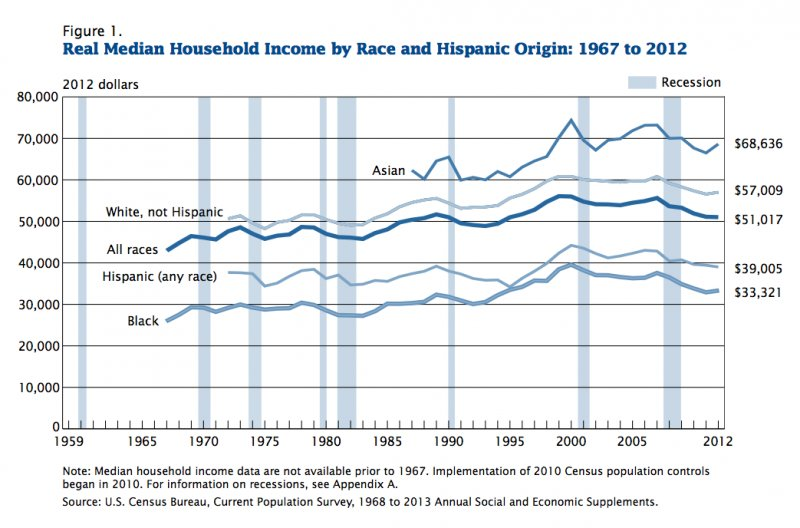
\includegraphics[width=14cm]{figures/Household_Income.png}
\caption[Real Median Household Income]{Real Median Household Income by Race and Hispanic Origin: 1967 -- 2012}
\label{fig:income}
\end{figure}

Social psychologists have developed their own theories of agents' racial preferences which further explains the mechanism of discrimination. Based on the empirical research of Henri Tajfel and John Turner, their theories shed light on segregation at the macro level\cite{tajfel79}. They define in-groups, or a group that one identifies with and is a member of, and out-groups, or groups that one is not a member of, to model prejudice and discrimination. Tajfel's Social Identity Theory claims that social categorizations systematize the social world and provide the agent with a system of self-reference. As such, the agent defines their identity and self-image from the social categories that he perceives himself belonging to. These categories may arise due to shared interests, shared racial categories, and enforcement by societal norms and authority, among other factors. Empirically, agents exhibit in-group favoritism, or a preference and affinity for one's in-group over the out-group even when the groups are arbitrarily constructed. This is potentially best shown in Jane Elliot's ``Blue eyes–Brown eyes" exercise\footnote{The Blue eyes–Brown eyes exercise aims to simulate discrimination. Specifically, a group of people was divided up based on their eye color. One group was deemed the privileged group and received benefits while the other group was treated poorly. Interaction between the two groups were discouraged and the non-privileged class had similar restrictions as African-Americans had before civil rights, such as being forced to sit in the back or drink from a different water fountain than Whites. It's worth noting that Elliot's exercise is not always successful in inducing discriminatory sentiment and has potential ethical issues (her sample was elementary school students). However, Elliot's work provides some evidence of the artificial nature of discriminatory sentiment.}. Moreover, agents exhibit out-group derogation, a phenomenon in which an out-group is perceived as being threatening to the members of a group. These empirically observed behaviors suggest the importance of incorporating class and racial preferences into the study of segregation. In-group members will strive to live with each other and move away from out-groups with different races, backgrounds, and interests. Regardless of the approach, we have a theory of why discrimination may exist at the individual level, manifested in preferences, and social level, manifested in segregation.

\section{Radical Cartography}

\begin{figure}[!h]
\centering
\begin{subfigure}{.5\textwidth}
  \centering
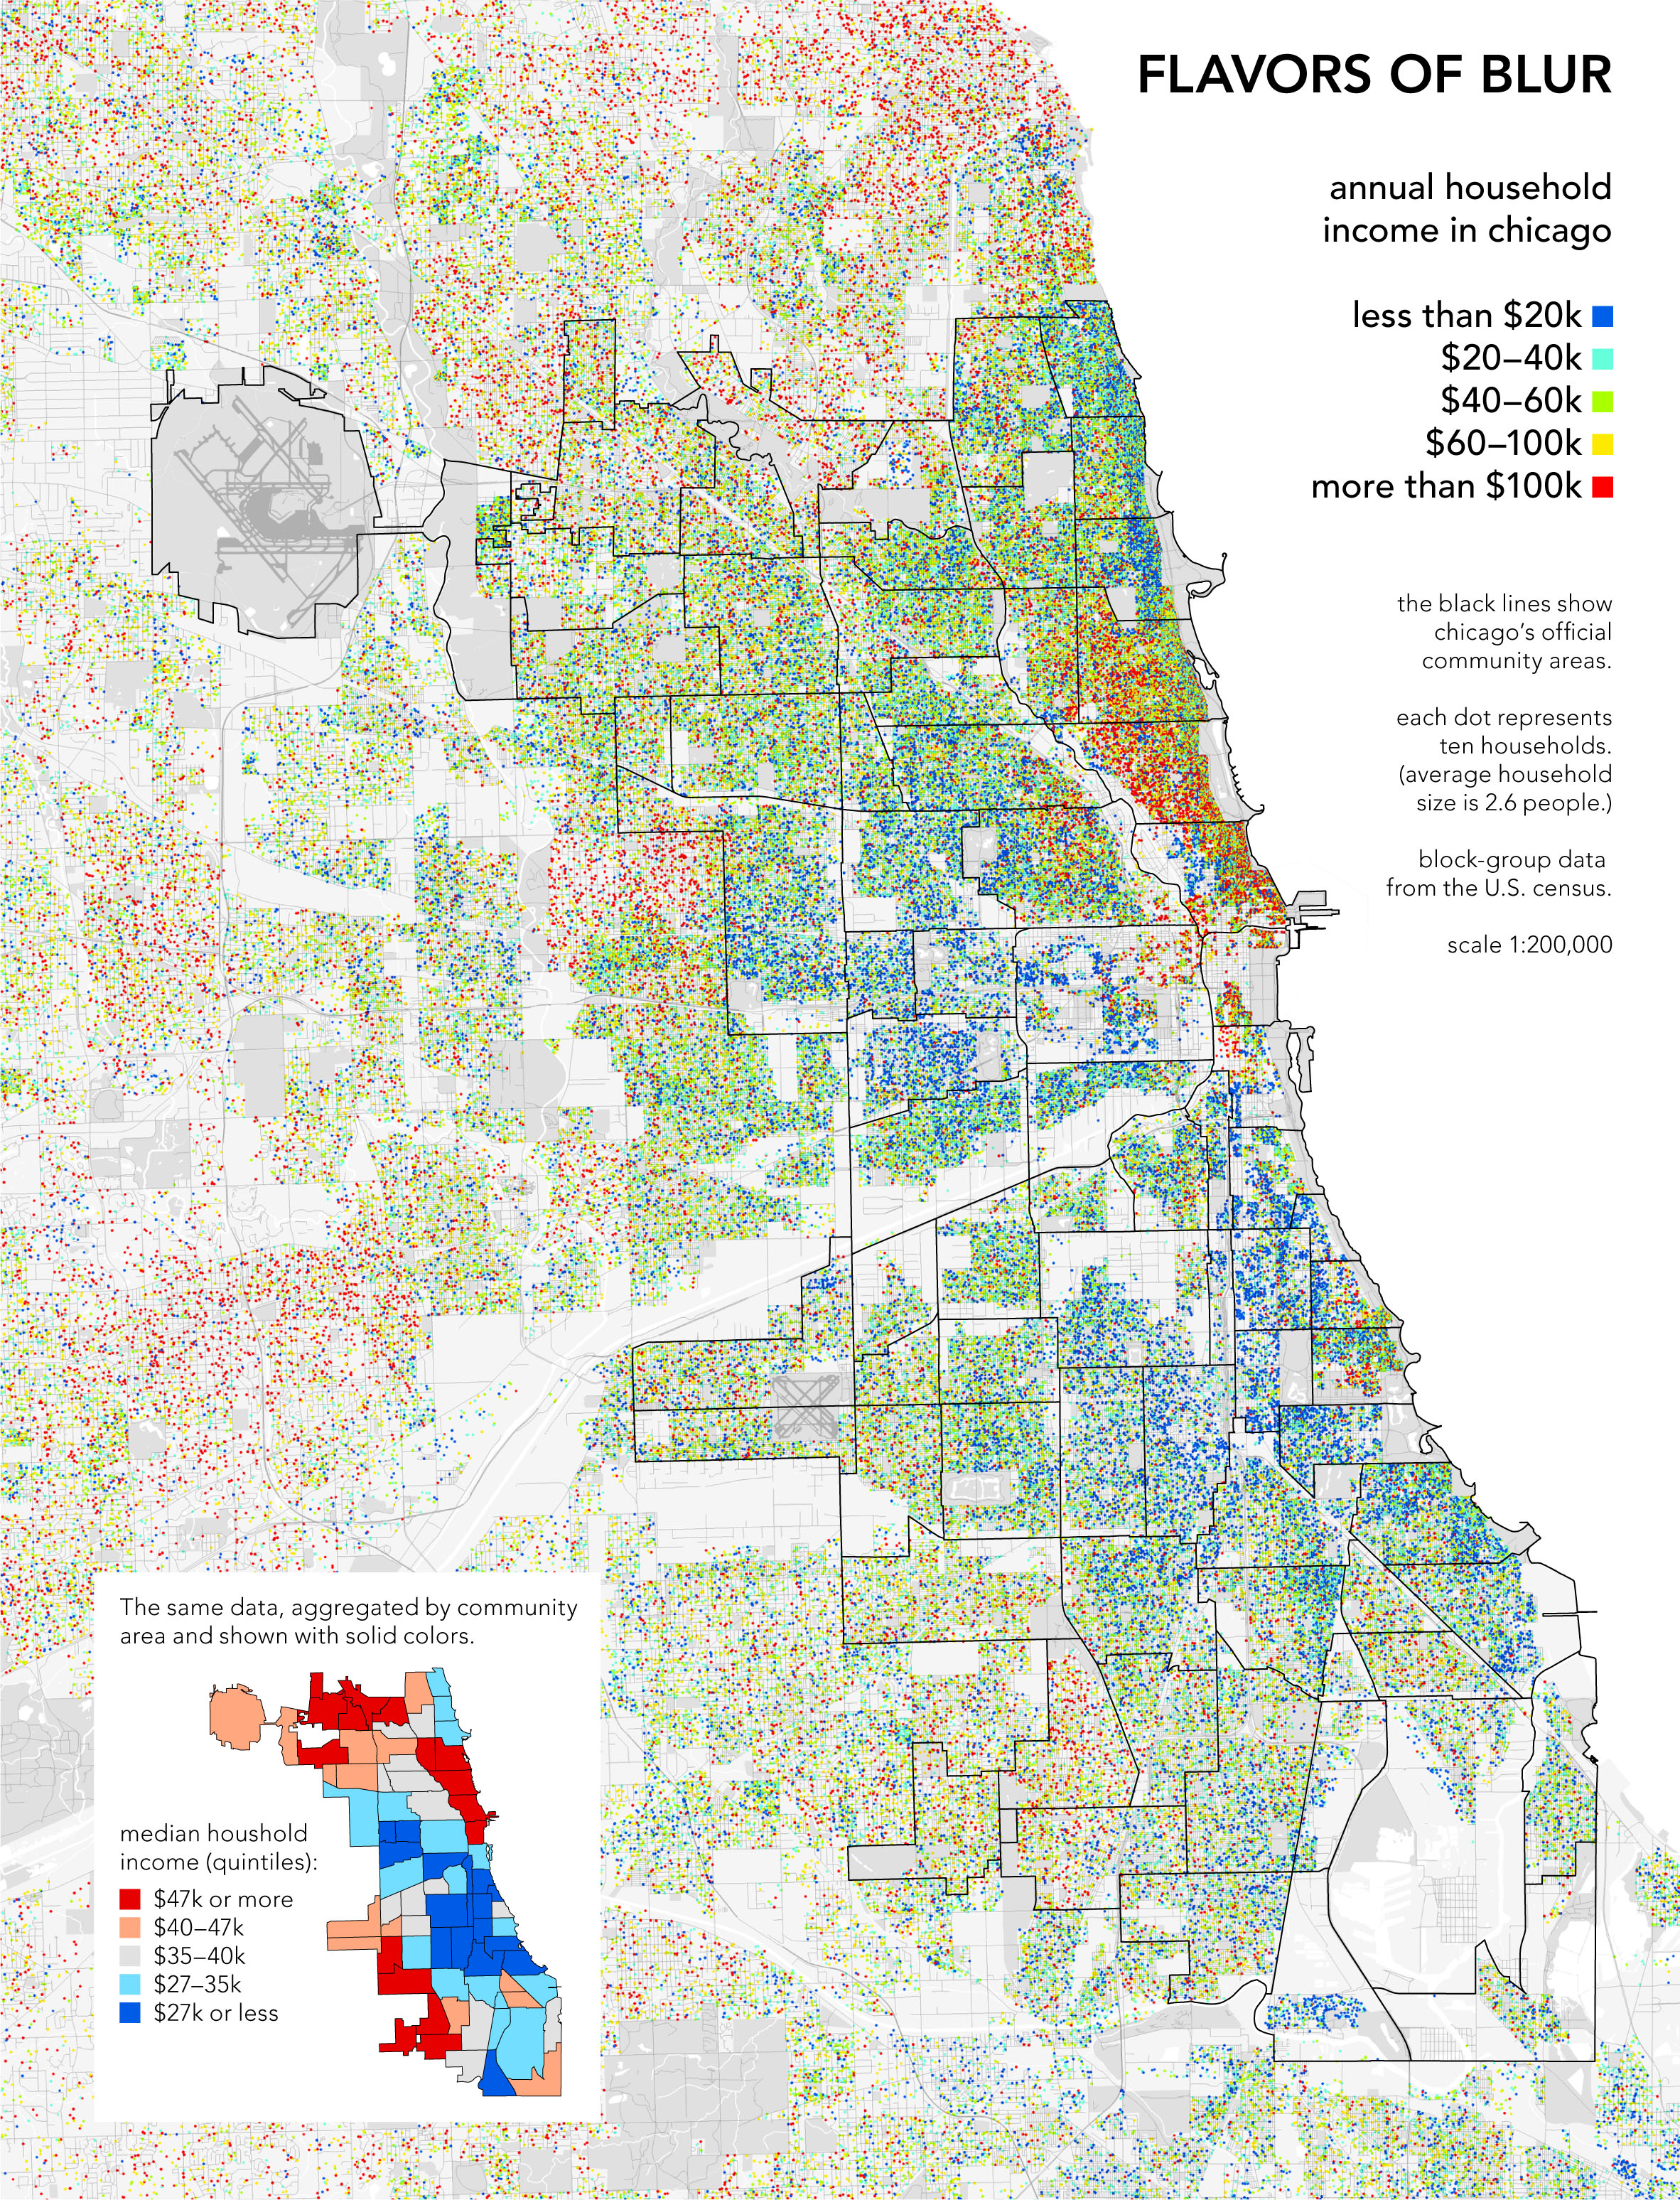
\includegraphics[scale=.35]{figures/chicagodots_income_big.jpg}
\end{subfigure}%
\begin{subfigure}{.5\textwidth}
  \centering
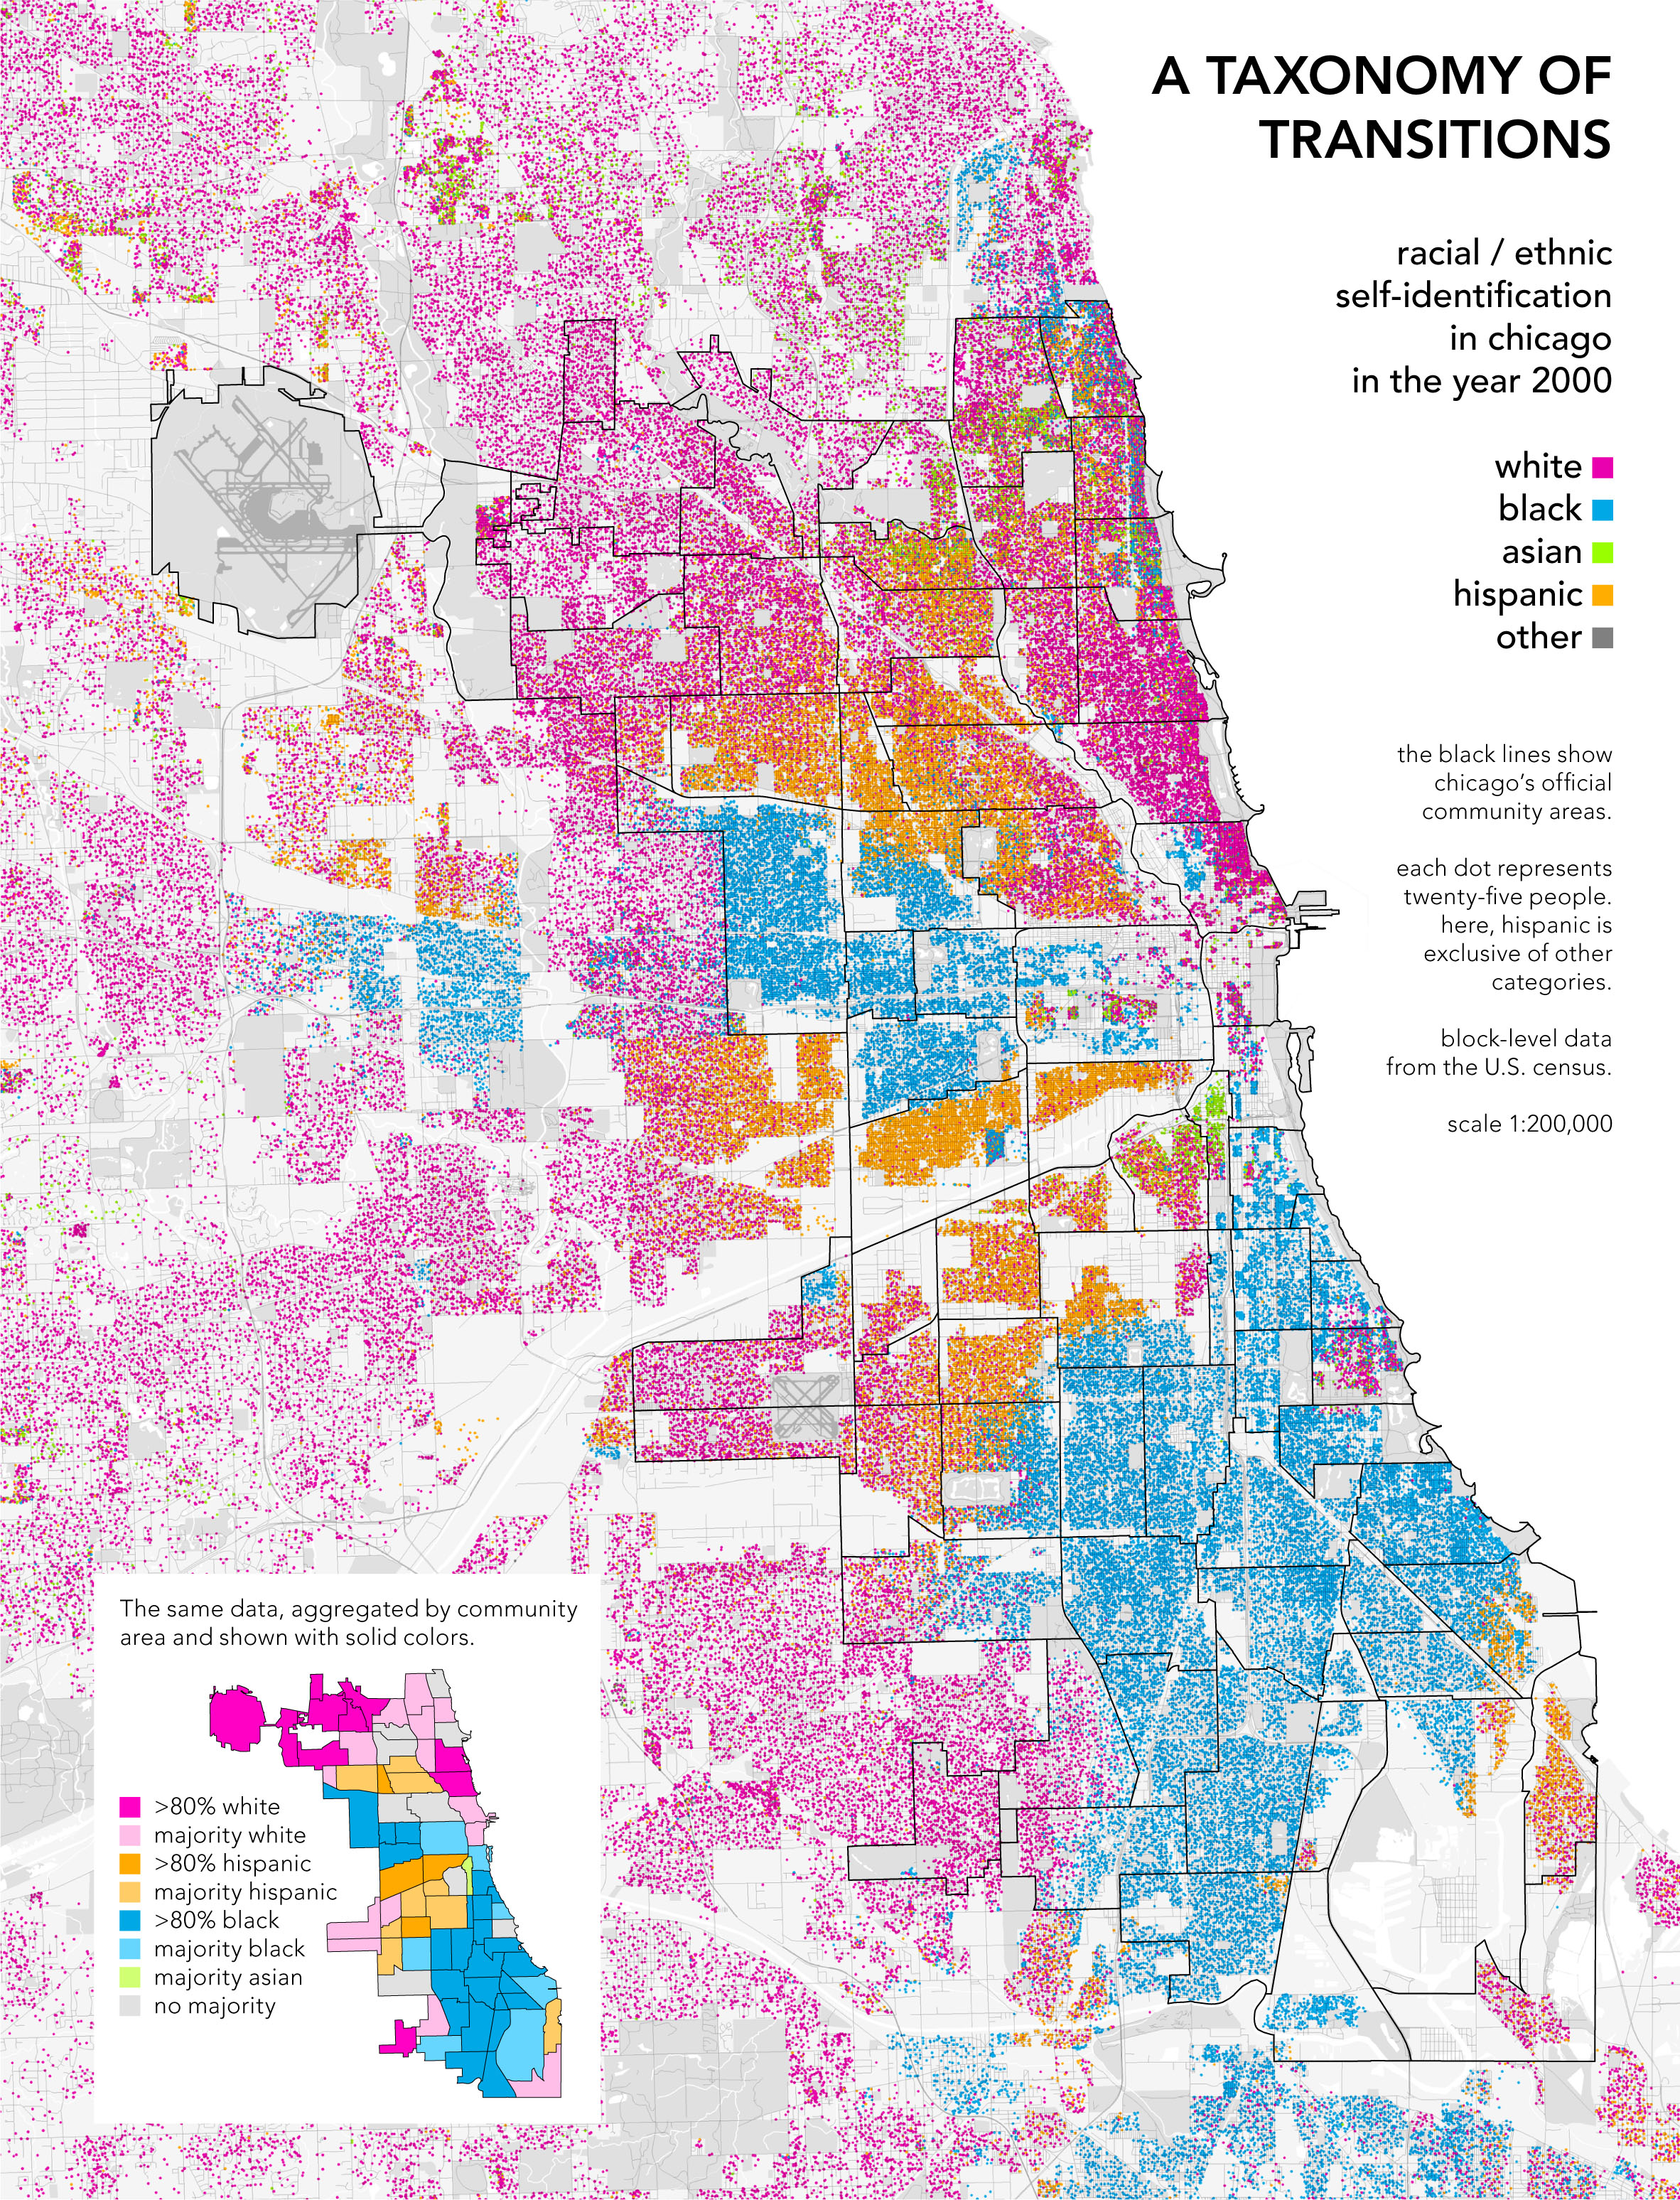
\includegraphics[scale=.35]{figures/chicagodots_race_big.jpg}
\end{subfigure}
\caption[Bill Rankin's Income and Race Maps of Chicago]{Bill Rankin's Income and Race distribution maps in Chicago (Source: Radical Cartography)}
\label{fig:rankin}
\end{figure}

Schelling's individual agent grids are best thought of as Pointillist maps, which have recently become popular with social scientists due to the work of cartographers like Bill Rankin. Unlike many other cartographers, Rankin focuses on destabilizing the traditional political undertones present in line-boundary maps. More precisely, he rejects the old mantra in cartography of strongly politically defined boundaries in favor of more measurable criteria. As Rankin writes: ``Boundaries lead a dual life: they are described as `imaginary lines,' often with no physical presence except on a map, but they also have very real effects on people, nature, and territory." \cite{rankin10}. Simply put, choosing which map to use influences not only our interpretation of the area but also influences the real development of the area itself. This is not a new idea, but Rankin and later Eric Fischer\footnote{Eric Fischer is a data artist and software developer at Mapbox. He has a photograph blog on Flickr with over 7.3k followers where he presents his racial Pointillist maps, among other things.} have become prominent in their respective fields with this work. 

Rankin creates a Pointillist style map where he represents agents as dots. This is in contrast to presenting the spacial demographics of a city by the ridge census tracts, which are a step removed from the individuals and may have political undertones in their form. The Pointillist style map allows the presentation of the agents to be more fluid and organic. The maps are technically more accurate as well because they emphasize each agent's location and identity rather than a superimposed framework. Comparing Rankin's maps with the traditional census map in figure \ref{fig:rankin}, the Pointiliist style map shows the smoothness and transition in greater detail. For purposes of this paper, this cartographic ideology allows us to use Tiebout's intuition of people ``voting with their feet" to attempt to capture the underlying economic phenomena rather than capturing the structure of the census blocs \cite{tiebout56}. Perhaps because Rankin is a cartographer and not a statistician, Rankin only presents qualitatively the difference between Pointillist style maps and the traditional variants\cite{rankin10}. He does not present an explicit error rate in the traditional census map versus a Pointillist map. This sort of analysis could potentially be useful to check whether this additional level of resolution would be beneficial in other scenarios. However in this case, there are clear gains and a simple integration to be had by integrating Rankin's radical cartography with a rigorous Schelling model.

\section{Tipping and Residential Segregation: A Unified Schelling Model}

Zhang (2011) \cite{zhang11} updates the Schelling model by both adding mathematical rigor and expanding upon some complications. Specifically, he models Schelling in a context of no racial discrimination wherein both Black and White agents prefer to live in 50-50 neighborhoods, and wherein socioeconomic disparities between white and black agents are completely eliminated. The mathematical rigor of the simulation allows for stronger proofs of the effects than Schelling's simulated examples. Zhang also clarifies some potentially nebulous definitions. Furthermore, Zhang facilitates extensions of the Schelling model, as now the richness of evolutionary game theory can be more easily implemented. As Zhang remarks, Young (1998) was the first to argue that the techniques developed in evolutionary game theory are useful for analyzing Schelling’s segregation and spacial models\cite{young98}. Foster and Young (1990) develop the concept of stochastic stability which is a rigorous analysis of long-run solutions in evolutionary game theory\cite{foster90}. Young (1998, 2001) presents a simple variation of the one-dimensional Schelling model on a ring\cite{young98,young01}. He shows that segregation tends to appear in the long run even though a segregated neighborhood is not preferred by any agent.

Zhang rigorously shows that stark segregation is a steady state in the situations he explores. The agents are in a Tragedy of the Commons game where no one or no set of agents is willing or able to take the necessary steps to ensure to maximize social or individual utility. Hence, the Nash equilibrium is not Pareto Optimal. It seems that unless there are very strong preferences in multiple agents for integration or a dictator-like social planner, segregation will persist in this model. Similarly, Zhang shows that the initial conditions are relatively invariant as both random start and `ghetto' starts lead to similar levels of segregation\footnote{In a random start, all the races are randomly mixed on the board. In a ghetto start, the Black population is concentrated at the center of the city.}. An important extension for Zhang is the inclusion of a housing market and heterogeneous agents in terms of wealth. This paper continues on that path.